
\begin{frame}[t, label=measurements]
    \frametitle{How Do We Make Measurements?}
    \begin{minipage}{0.7\textwidth}
        \redout<8->{\textbf{In-Situ Measurements}: Go there and see!}
        \begin{itemize}
            \item<2-> \alt<3->{\redout{Satellites?}}{Satellites?} \quad \visible<3->{\textit{Atmosphere too dense!}} 
            \item<4-> \alt<5->{\redout{Balloons?}}{Balloons?} \ \quad \visible<5->{\textit{Too high up!}}
            \item<6-> \alt<7->{\redout{Rockets?}}{Rockets?} \ \ \quad \visible<7->{\textit{Expensive! Infrequent! Poor coverage!}}
        \end{itemize}
    \end{minipage}
    \begin{tikzpicture}[remember picture, overlay]
        \node<2->[anchor=north east] (satellite) at ([xshift=-3.25cm, yshift=-1cm]current page.north east) {
            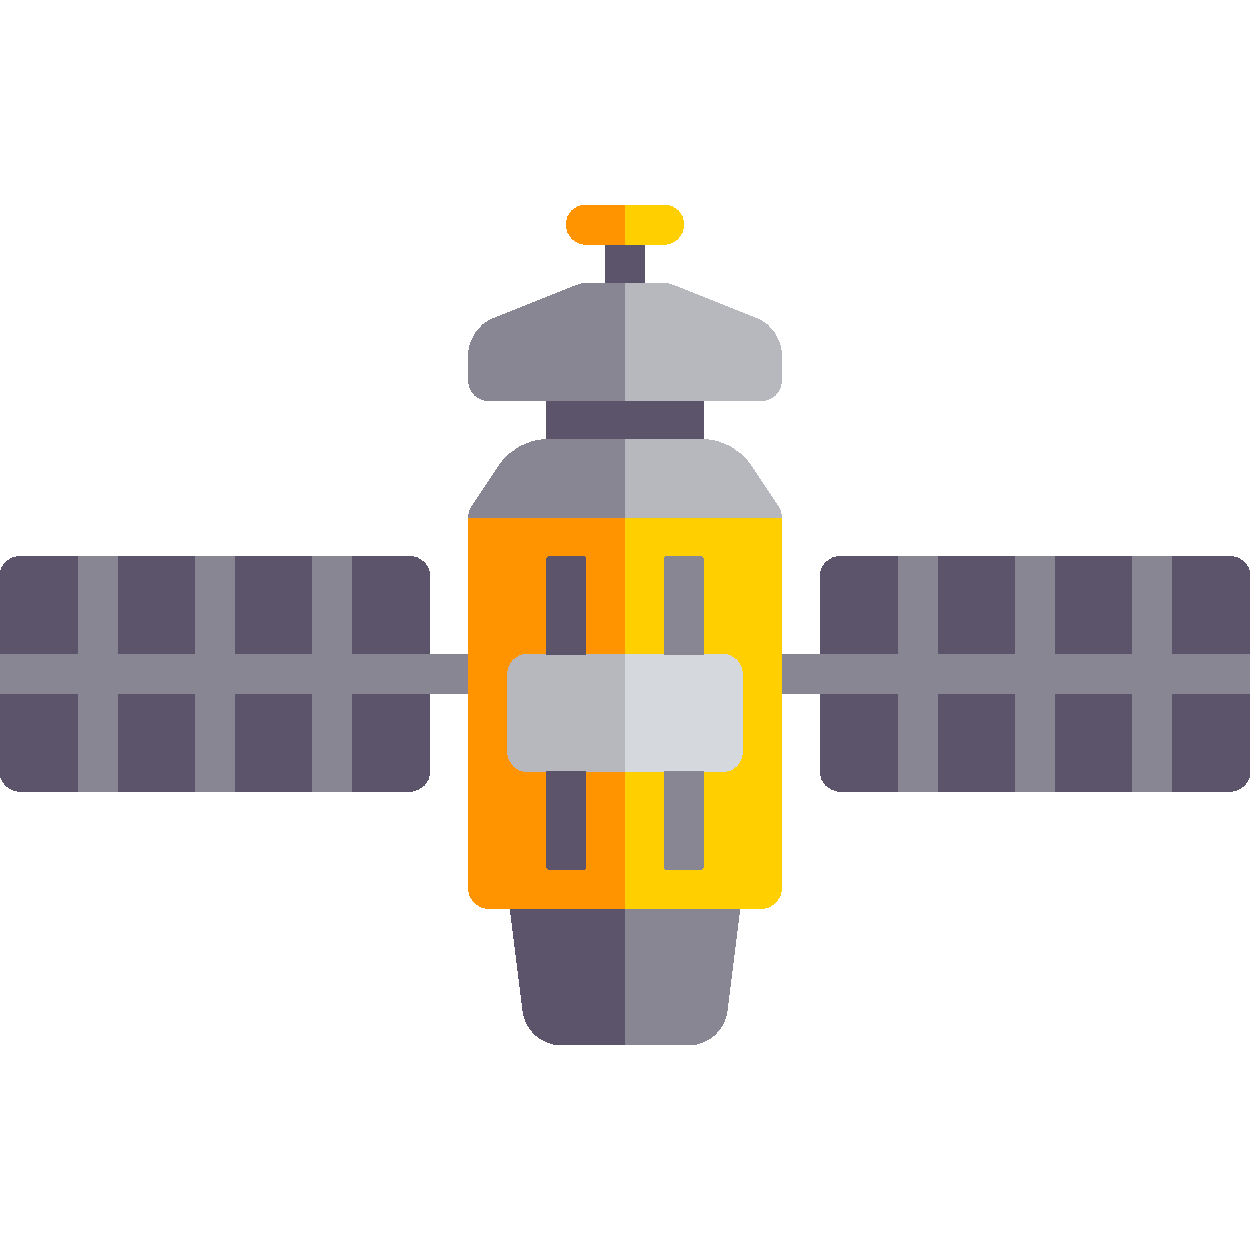
\includegraphics[width=1.5cm]{img/satellite.pdf}
        };
        \node<3-> at ([xshift=-0.5cm, yshift=-0.5cm]satellite.north east) {
            
\includegraphics[width=0.5cm]{img/fire.pdf}
        };
        \node<3-> at (satellite.center) {
            
\includegraphics[width=1cm]{img/no.pdf}
        };

        \node<4->[anchor=north east] (balloon) at ([xshift=-0.5cm, yshift=-2cm]current page.north east) {
            
\includegraphics[width=1.25cm]{img/balloon.pdf}
        };
        \node<5-> at ([xshift=-0.4cm, yshift=-0.4cm]balloon.north east) {
            
\includegraphics[width=0.5cm]{img/pop.pdf}
        };
        \node<5-> at (balloon.center) {
            
\includegraphics[width=1cm]{img/no.pdf}
        };

        \node<6->[anchor=north east] (rocket) at ([xshift=-2.5cm, yshift=-2.75cm]current page.north east) {
            
\includegraphics[width=1.25cm]{img/rocket.pdf}
        };
        \node<7-> at ([xshift=-0.25cm, yshift=0.35cm]rocket.south east) {
            
\includegraphics[width=0.75cm]{img/money_bag.pdf}
        };
        \node<7-> at (rocket.center) {
            
\includegraphics[width=1cm]{img/no.pdf}
        };

        \node<9->[anchor=south east] at ([xshift=0cm, yshift=0.5cm] current page.south east) { 
            \animategraphics[loop, autoplay, height=0.42\textheight]{24}{img/radar_gif/radar_}{01}{97}    
        };
    \end{tikzpicture}

    \uncover<9->{\textbf{Remote Sensing}: Look and guess from afar

    Radar uses \alert{electromagnetic waves} to probe far away objects
    \begin{itemize} \small \vspace{-0.5\baselineskip}
        \item Signal round trip time \(\xrightarrow[]{}\) \alert{distance}
        \item Doppler shift \(\xrightarrow[]{}\) \alert{speed} 
    \end{itemize}
    \begin{textblock*}{1cm}(\paperwidth - 1cm, \paperheight - 1cm)
        {\fontsize{5}{5.4}\selectfont \textcolor{black}{Credit: \cite{wolff_RangeDistanceMeasurement_}}}
    \end{textblock*}}
\end{frame}
